\documentclass[12pt]{article}

\usepackage{epsfig}
\usepackage{rotating}
\usepackage{lscape}
\usepackage{amsfonts}
\usepackage{amssymb}
\usepackage{theorem}
\usepackage{amsmath}
\usepackage{graphicx}
\usepackage{citesort}
\usepackage{float}
\usepackage{color}
\usepackage{array}
\usepackage{color}
\usepackage{array}
\usepackage{float}
\usepackage{url}
\usepackage{setspace}
%\usepackage{amsmath,amsfonts,amssymb,cite,array,graphicx}
\usepackage{algorithm}
\usepackage{algpseudocode}
\usepackage{multicol}
\usepackage{calc}
\usepackage{caption}
\usepackage{subcaption}

\textwidth=17.36cm
\textheight=23.90cm
\hoffset=-2.37cm
\voffset=-2.5cm
\parskip=1pt

\renewcommand{\rmdefault}{ptm}

\newtheorem{definition}{Definition}[section]
\newtheorem{theorem}{Theorem}[section]
\newtheorem{corollary}{Corollary}[section]
\newtheorem{lemma}{Lemma}[section]
\newtheorem{remark}{Remark}[section]


\date{\small\today} \title{Speeding Up A* Search Through Symmetry Reduction} \author{Jeffrey Picard} 
%\doublespacing

\begin{document}

\maketitle

\begin{abstract}
There is wide usage in AI, robotics and video games of pathfinding on uniform cost grids. Therefore the ability the speed up the search time of algorithms like A*
which is ubiquitous in this area is an extremely relevant one to the field. Some approaches, such as hierarchical methods, have shown success in accomplishing 
this but at the cost of optimality. A recent idea for another method to speed up A* search on uniform cost grids, called ``Symmetry Reduction'' or 
``Symmetry Breaking'' is to detect and remove symmetric paths from the search space and thus save node generations and time. Symmetric paths are defined as 
paths which start and end in the same location, have the same length and may be transformed into each other through a reordering or permutations of the 
vertices that make up the path, the vertices being lengths of the path moving in only one direction. In this paper two different methods of speeding up A* 
search through symmetry reduction, Jump Point Symmetries (JPS) and Rectangular Symmetry Reduction (RSR), that maintain optimality are explored. Empirical
results show significant speedup over Vanilla A* using both algorithms and JPS dominating RSR. A proof is also given that JPS may be extended to a slightly
larger set of problems than orginally considered in \cite{Har2011}.
%Some considerations for implementation are also mentioned.
%and it is shown that each method may be extended to slightly larger set of problems than previously considered.
\end{abstract}


% main text
\section{Introduction}
The two methods of symmetry reduction that are explored are Rectangular Symmetry Reduction (RSR) and Jump Point Symmetries (JPS)\cite{Har2011,Har2010}. 
RSR identifies large empty
rectangles in the search space and removes them leaving only the exterior nodes and inserting ``macro edges'' so an agent may jump across the space in 
order to preserve optimality. This method was implemented by this author on a 4-connected grid map. JPS by contrast is an online method that recursively prunes 
all neighbors of the current node that can be optimally reached by the node's parent without going through the current node. The recursion ends when the path 
is blocked or at the edge of the map or a node is found that has a neighbors $n$ which cannot be reached optimally by the node's parent. 
Therefore the path should either not be considered or the optimal path to $n$ is through the current node. This algorithm was implemented on an 8-connected
grid map by this author. JPS as it was first introduced in\cite{Har2011} was only stipulated to work for a single goal. In this paper, it is shown that this 
is easily also extended to allow multiple goals and optimality is maintained. An empirical performance analysis of the algorithms is also provided.
	
\section{Implementation}
In the JPS algorithm, before a node is expanded, its neighbors are pruned according to two rules which determine which neighbors may not be reached
optimally from the node's parent without traversing that node. The idea behind both rules are the same but a slightly different constraint is enforced
for diagonal moves as opposed to straight ones. 

The result of these pruning rules is that for any straight move there is one neighbor that a node will always have, assuming it isn't blocked or 
off the grid. In Figure \ref{sm:1} the node whose neighbors are being considered is labaled X and the natural neighbor is colored in green. To consider 
straight moves in other directions the diagram merely need be rotated. In a similar fashion there will be three neighbors that a diagonal move will always 
have. These can be seen Figure \ref{dm:1} for which the same coloring scheme and comment about rotating the diagram to produce other moves also apply. 
In addition, in order to check for forced neighbors there is only ever need to check to see if two neighbors are blocked. In the straight movement case
the nodes to either side perpendicular to the direction of movement are checked and if either is blocked the neighbor at a 45 degree angle to that side
of the node is forced. In Figure \ref{sm:2} the blocked node is colored in red and the forced node in blue. The idea is again similar in the diagonal case 
with the neighbors perpendicular to the direction of movement, this time at 45 degree angles from the point inbetween X and it's parent, the ones that are
check to see if they are blocked. In Figure \ref{dm:2} an example is provided with the same coloring scheme as before.

In considering the specifics of these rules there are a few elements of notation worth mentioning. $p(x)$ is the parent of the current node $x$, 
whose neighbors we are pruning. The brackets $<...>$ indicate a path through the specified nodes and $\setminus$ is the set minus operator. This paper
follows the same notational conventions for these rules as \cite{Har2011}.
For straight moves any neighbor node $n$ which satisfies the following inequality is pruned.

$len( <p(x),...,n> \setminus x ) \le len( <p(x),x,n> )$

That is, any neighbor node which may be reached from the parent of x -- without going through x -- is pruned. For diagonal moves the inequality simply
becomes strictly less than, thus when moving diagonally any neighbor node $n$ such that the following inequality is satisfied is pruned.

$len( <p(x),...,n> \setminus x ) < len( <p(x),x,n> )$


\begin{figure}
  \begin{subfigure}[b]{.5\linewidth}
    \caption{Natural neighbors of a straight move.}\label{sm:1}
    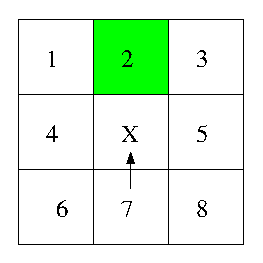
\includegraphics[scale=1]{figures/straight_movement_1.eps}
  \end{subfigure}
  \begin{subfigure}[b]{.5\linewidth}
    \caption{Forced neighbor of a straight move.}\label{sm:2}
    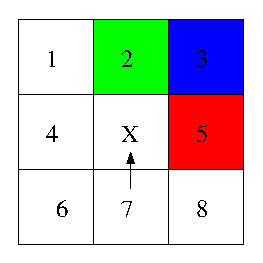
\includegraphics[scale=1]{figures/straight_movement_2.eps}
  \end{subfigure}
  \caption{Straight movement neighbor pruning}\label{sm}
\end{figure}

\begin{figure}
  \begin{subfigure}[b]{.5\linewidth}
    \caption{Natural neighbors of a diagonal move.}\label{dm:1}
    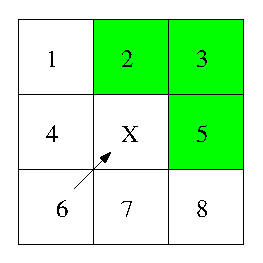
\includegraphics[scale=1]{figures/diag_movement_1.eps}
  \end{subfigure}
  \begin{subfigure}[b]{.5\linewidth}
    \caption{Forced neighbors of a diagonal move.}\label{dm:2}
    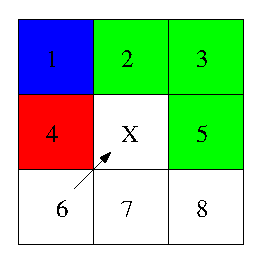
\includegraphics[scale=1]{figures/diag_movement_2.eps}
  \end{subfigure}
  \caption{Diagonal movement neighbor pruning}\label{dm}
\end{figure}

\section{Extending JPS To Multiple Goals}
As noted earlier when JPS was introduced by Harabor is was only considering a single goal. In Algorithm \ref{IdSuccessors} and Algorithm \ref{jump} 
the pseudo code from \cite{Har2011} is provided for implementing JPS. Note that the start goal's neighbors are not pruned. With this implementation 
alone there are cases where the algorithm
will not return a solution for a map with multiple goals. It is assumed that the goal is simply replaced by a goal list and line four in 
Algorithm \ref{jump} is changed to \textbf{if} $n \in g$ \textbf{then}. A simple example of such a case is provided in Figure \ref{bad_jps}. 
Here the agent is indicated by an ampersand symbol and the goals by asterisks. 
First the start node is expanded and nodes 2, 4 and 5 are selected as neighbors. The jump algorithm then
progresses to tiles 3, 7 and 9. When it reaches 7 null is returned and when 3 and 9 are reached they are returned as goals. However all of the neighbors
of 3 and 9 are then pruned when they are expanded and no further search is done and the algorithm fails to find a path. Note that JPS will find all the of
the goals individually. Since each goal has an optimal path from the start, this follows trivially from the proof in\cite{Har2011} that JPS will return
an optimal path to a goal.

\begin{figure}
\begin{center}
  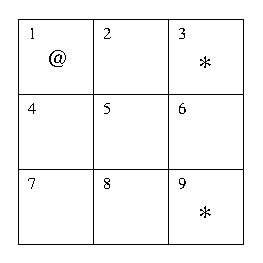
\includegraphics[scale=1]{figures/JPS_multiple_goals_counter_example.eps}
  \caption{A simple grid world JPS cannot find a path for.}\label{bad_jps}
\end{center}
\end{figure}

The solution to this is simply treat each goal reached -- until all the goals have been reached -- as another start point and not
prune any of its neighbors. This will in effect restart the JPS algorithm from each intermediate goal while still preserving the information within A*
about the current distance traveled so far and any heuristics that are calculated.

$Proof.$
For any grid with $n$ goals $G = \{ g_{0}, g_{1}, ..., g_{n-1} \} $, all reachable, there is an optimal path $\pi$ that takes $n$ optimal subpaths 
$P = \{ \pi_{0}, \pi_{1}, ..., \pi_{n-1} \}$ in an optimal order with $\pi_{i}$ the path from $g_{i-1}$ to $g_{i}$. Note $g_{-1}$ is the start position.
JPS will find an optimal path from the start to each goal $g_{i} \in G$. 
Since $\pi_{0}$ is the first optimal subpath it begins at the start and ends at the first goal $g_{0}$. Therefore $\pi_{0}$ will be found. 
Now assuming an arbitrary goal $g_{i} \in G$ has been found through the optimal subpath $\pi_{i}$, restarting the JPS algorithm from that goal will find 
the optimal subpath $\pi_{i+1}$ to goal $g_{i+1}$. Therefore the optimal path $\pi$ will be found. $\Box$

\begin{algorithm}
\caption{Identify Successors}\label{IdSuccessors}
\begin{algorithmic}[1]
\Require $x$: current node, $s$: start node, $g$: goal
\State $successors(x) \gets \emptyset$
\State $neighbors(x) \gets prune(x,neighbors(x))$
\ForAll{$n \in neighbors(x)$ }
  \State $n \gets jump(x,direction(x,n),s,g)$
  \State add $n$ to $successors(x)$
\EndFor
\end{algorithmic}
\end{algorithm}

\begin{algorithm}
\caption{Function $jump$}\label{jump}
\begin{algorithmic}[1]
\Require $x$: initial node, $\vec{d}$: direction, $s$: start $g$: goal
\State $n \gets step(x,\vec{d})$
\If{ $n$ is an obstacle or is outside the grid }
  \State \Return $null$
\EndIf
\If{$n = g$}
  \State \Return $n$
\EndIf
\If{ $\exists n' \in neighbors(n)$ s.t. $n'$ is forced}
  \State \Return $n$
\EndIf
\If{$\vec{d}$ is diagonal}
  \ForAll{$i \in \{1,2\}$}
    \If{$jump(n,\vec{d_{i}},s,g)$ is not $null$}
      \State \Return n
    \EndIf
  \EndFor
\EndIf
\end{algorithmic}
\end{algorithm}

\section{Results}
The two symmetry reduction algorithms were tested on maps from the video game Dragon Age Two available from movingai.com.
In Figure \ref{rsr_speedup} it can be seen that the time and node generation speedup were modest and even started below one for RSR. 
These results are similar to the ones from \cite{Har2010}. In Figure \ref{jps_speedup} much more significant time and node generation speedup
can be seen for JPS. The time speedup in again similar although more exaggerated than was seen in \cite{Har2011}. This is probably due to Python
being used to implement the A* algorithm. Node generation speedup seen in Figure \ref{jps_speedup:nodes} was very significant. This metric was not
plotted in \cite{Har2011} so there is nothing to compare against here.

\begin{figure}
  \begin{subfigure}[b]{.5\linewidth}
    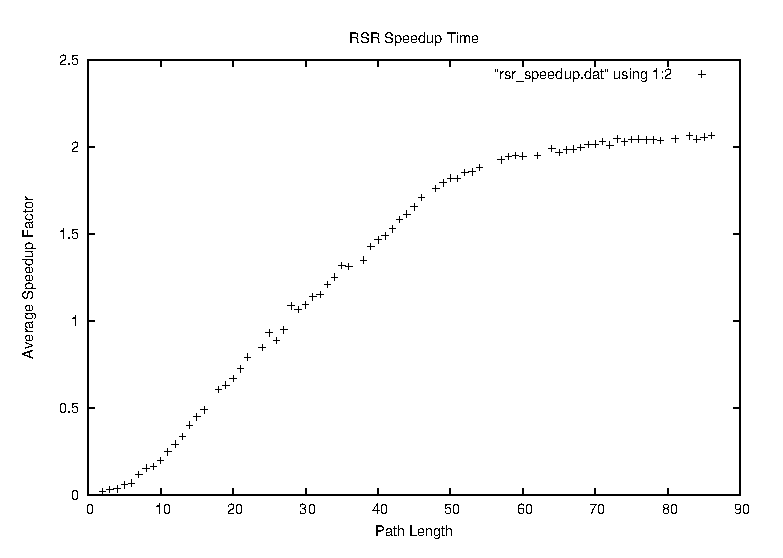
\includegraphics[scale=0.6]{figures/rsr_speedup_time.eps}
    \caption{RSR Time Speedup}\label{rsr_speedup:time}
  \end{subfigure}
  \begin{subfigure}[b]{.5\linewidth}
    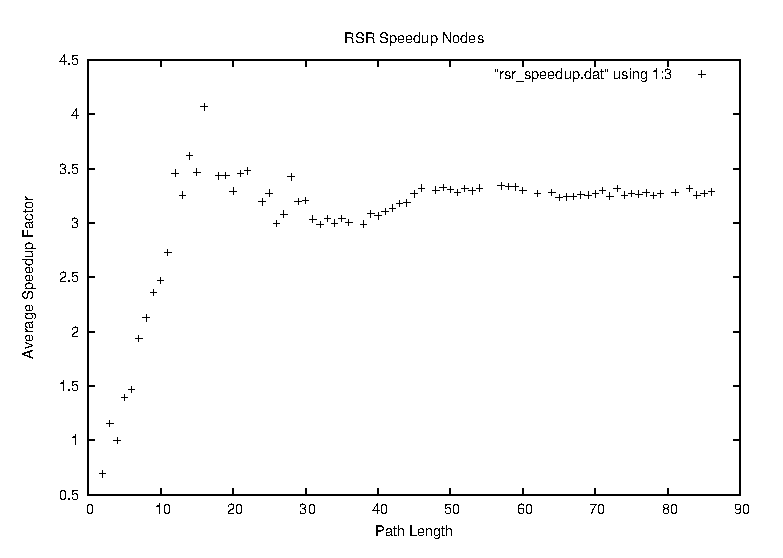
\includegraphics[scale=0.6]{figures/rsr_speedup_nodes.eps}
    \caption{RSR Nodes Speedup}\label{rsr_speedup:nodes}
  \end{subfigure}
  \caption{RSR Speedup}\label{rsr_speedup}
\end{figure}

\begin{figure}
  \begin{subfigure}[b]{.5\linewidth}
    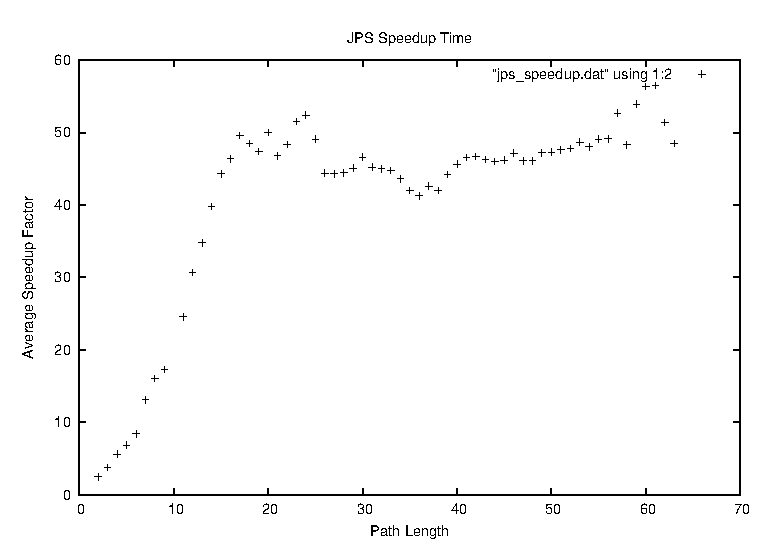
\includegraphics[scale=0.6]{figures/jps_speedup_time.eps}
    \caption{JPS Time Speedup}\label{jps_speedup:time}
  \end{subfigure}
  \begin{subfigure}[b]{.5\linewidth}
    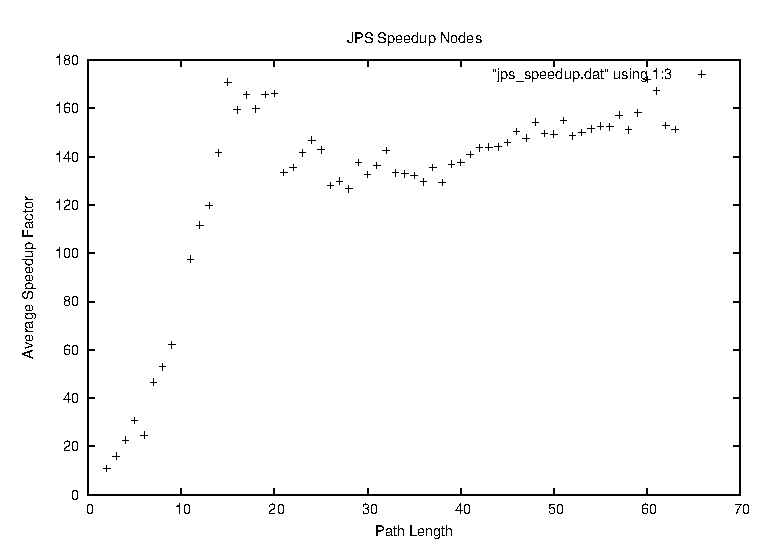
\includegraphics[scale=0.6]{figures/jps_speedup_nodes.eps}
    \caption{JPS Nodes Speedup}\label{jps_speedup:nodes}
  \end{subfigure}
  \caption{JPS Speedup}\label{jps_speedup}
\end{figure}

\newpage

\section{Conclusion}
Two methods for speeding up vanilla A* search that exploited symmetric paths and maintained optimality were explored and empirical 
results were gathered. While both methods did exhibit an ability to increase the performance of A*, RSR is very dependent on large empty 
spaces and has additional memory overhead due to the need to store macro edges. JPS also showed performance that dominated that of RSR
in every case. Some practical considerations for implementing JPS were discussed pertaining to
how to prune neighbors. Also a proof was provided that shows JPS may easily be extended to domains where multiple goals need to be reached.

%\section{Further Work}

\bibliographystyle{elsarticle-num}
\bibliography{main_ai}

\end{document}
